\documentclass[thesis.tex]{subfiles}
\begin{document}
\chapter{The application of AppPAL to BYOD policies}
\label{chap:byod}

Many employees bring their personal mobile devices to work. To control the
access these devices have, 70\% of companies publish \emph{bring your own
  device} (BYOD) policies~\cite{schulze_byod_2016}. These BYOD policies are
written documents for employees to read and follow. They describe steps to take
to secure devices appropriate to the workplace. The policies say how employees
should access data, and who should authorise decisions.

Companies have a variety of means to implement their policies. Some companies
may trust employees to follow the rules on their own. Alternatively \emph{Mobile
  Device Management} (MDM) software can implement part of the policies: packages
such as IBM's MaaS360 and Blackberry's BES~\cite{_ibm_????,_secure_????} can
configure devices to restrict functionality and manage apps.

Commercial tools are limited in what polices they can enforce. Some tools can
only enable simple on-off configuration settings, and ban explicitly
black-listed apps. More sophisticated systems can use app-rewriting to recompile
apps to tunnel traffic through a VPN, or geofencing to apply policies in
predefined areas. These tools are not infallible. One survey found that 50\% of
companies with MDM software still had non-compliant devices in their
networks~\cite{mobileiron_security_labs_q4_2015}. Whilst app wrapping can
protect some apps, in general it is ineffective~\cite{hao_effectiveness_2013}.

\section{Overview of five BYOD policies}

Five policies were selected from a variety of domains.
These were chosen as they cover a range of different policy styles, and
concerns.

\begin{itemize}
\item The first is the \emph{Security Policy Template: Use of Handheld Devices
    in a Corporate Environment}, published by the SANS
  Institute~\cite{nicholas_r._c._guerin_security_2008}. This policy is a
  hypothetical policy published to help companies mitigate the threats to
  corporate assets caused by mobile devices. Companies are expected to modify the
  document to suit their needs. The policy is general; not specific to any
  particular industry, device, or country's legislation.
\item The second is taken from the
  \ac{HiMSS}~\cite{healthcare_information_and_management_systems_society_mobile_2012};
  a US non-profit company trying to improve healthcare through IT. The \ac{HiMSS}
  policy is relatively short and contains concerns specific to healthcare
  scenarios. It is written as a contract the users agree to follow. In contrast,
  every other policy we looked at is written as an organisation imposing rules on
  users they should follow to ensure compliance. The policy is designed as a
  sample agreement for a system trying to manage personal mobile devices in a
  healthcare environment.
\item The third is taken from a British hospital
  trust~\cite{kennington_mobiles_2014} and describes the BYOD scheme used in
  practice at the hospital.  The policy is broad and also covers rules for
  corporately owned devices.  This policy also briefly describes how devices
  should interact with patients.
\item Finally, we looked at two simpler policies from The University of
  Edinburgh~\cite{williamson_bring_2015} and a company specialising in emergency
  sirens~\cite{code3pse.org_sample_????}. These policies are simpler, and shorter
  than the other policies we looked at comprised of much more general rules.
\end{itemize}

Each of the policies is split into a series of rules and requirements employees
should follow. Typically the policy is written describing what employees should
do and what will happen under certain circumstances. For example the NHS policy
states that:

\begin{policyrule}{NHS}
  In the event of loss of the device, all data including apps will be wiped. The Trust
  is not responsible for reimbursement of any costs for personally purchased apps.
\end{policyrule}

The Siren policy matches this style, stating what conditions will lead to the
company wiping an employees device:

\begin{policyrule}{Sirens}
The employee’s device may be remotely wiped if: $\bullet$ The device is lost or
stolen. $\bullet$ The employee terminates his or her employment. $\bullet$ IT
detects a data or policy breach, a virus or similar threat to the security of
the company’s data and technology infrastructure.
\end{policyrule}

In contrast the \ac{HiMSS} policy is written as a contract where the user states
what they will do.

\begin{policyrule}{HiMSS}
  I agree that the PDA/Smartphone can be wiped by XYZ Health System upon the
  decision of XYZ Health System management and understand that it will delete all
  data including personal files.
\end{policyrule}

The SANS policy is mostly written in the same style as the NHS policy.  It is
written as a hypothetical policy that a company might use as the basis for their
own policy, however it sometimes says things that seem like advice to an IT
department implementing the policy.  It also For example:

\begin{policyrule}{SANS}
   A corporate mobile device management solution SHALL feature remote device
   wiping (or possibly only blocking) mechanism for all devices accessing
   corporate internal networks.
\end{policyrule}

The SANS policy also distinguishes between rules that should always be followed (SHALL),
and those that may depend on a specific business's situation (SHOULD).

\begin{policyrule}{SANS}
  Basically, sentences using the verb ``SHALL'' are mandatory requirements
  applying to practices with high probability of putting the business at risk,
  whereas ``SHOULD'' means that the policy needs to be applied according to the
  business’s specific situation.
\end{policyrule}

The Edinburgh policy takes this even further. Rules are grouped by type of
device, and are given a security marking.  High and mediu,m risk users are
expected to follow everything, and low risk users are expected to at least
consider following the rules marked with a nabla.  For example the
rule for remote wiping devices is grouped with the rules specific to mobile
devices and tablets, and is marked with a triangle.

\begin{policyrule}{Edinburgh}
  $\nabla$ Configure your device to enable you to remote-wipe it should it become lost.
\end{policyrule}


\section{Review of MDM software}

To implement policies companies can use \ac{MDM} software to try and implement
their rules.  \ac{MDM} solutions are offered by a many companies, including IBM
(MaaS360), VMware (AirWatch) and MobileIron; however they all offer a
comparable set of features, namely:
\begin{enumerate}
\item App wrapping; where an app is rewritten to offer some addtional security
  or network properties. This is often limited to routing all the app's
  network traffic through a VPN.
\item Basic security configuration; where security settings can be turned on and
  off to require encryption (for example) on a device.
\item Provisioning; where IT departments can install and update apps and
  their configuration files. Email and LDAP configuration is common.
\item A curated app store; where IT departments can white or black list apps.
\end{enumerate}

The features of 9 competing MDM packages identified by a Gartner report are
summarised in \autoref{tab:mdm-capabilities}~\cite{rob_smith_magic_2016}.  Most
of the tools link to the report on their homepages as the report lists \emph{every} tool as
either \emph{visionary}, \emph{leading}, or \emph{niche player}.\footnote{The
  table summarises the visionary and leading MDM packages.}  In practice all the
tools are very similar with the chief difference being the UI as well as some
extra features only certain tools support.

\begin{table}\centering\sffamily\footnotesize
  \begin{tabular}{l c c c c c c c c c}
    \toprule
    Feature                           & \rb{MaaS360} & \rb{Blackberry BES} & \rb{MobileIron} & \rb{Citrix XenMobile} & \rb{VMWare AirWatch} & \rb{Microsoft} & \rb{SOTI MobiControl} & \rb{Sophos} & \rb{Landdesk} \\
    \midrule
    Antivirus                         &              &                     &                 &                       &                      &                &                       & \cmark      &               \\
    App selection/store/management    & \cmark       & \cmark              & \cmark          & \cmark                & \cmark               & \cmark         & \cmark                & \cmark      & \cmark        \\
    App wrapping/modification         &              & \cmark              & \cmark          & \cmark                & \cmark               & \cmark         &                       & \cmark      & \cmark        \\
    Authentication                    & \cmark       & \cmark              & \cmark          & \cmark                & \cmark               & \cmark         & \cmark                &             &               \\
    Compliance reporting              & \cmark       & \cmark              & \cmark          & \cmark                & \cmark               & \cmark         & \cmark                & \cmark      &               \\
    Device configuration              & \cmark       & \cmark              & \cmark          & \cmark                & \cmark               & \cmark         & \cmark                &             & \cmark        \\
    Email/Calendar/Contacts/Documents & \cmark       & \cmark              & \cmark          & \cmark                & \cmark               & \cmark         & \cmark                & \cmark      & \cmark        \\
    Feature Restrictions              & \cmark       & \cmark              &                 &                       & \cmark               & \cmark         &                       &             &               \\
    Licence distribution              &              & \cmark              &                 &                       &                      &                &                       &             &               \\
    Location based settings           & \cmark       &                     &                 &                       & \cmark               &                &                       &             &               \\
    Network configuration             & \cmark       & \cmark              & \cmark          & \cmark                & \cmark               & \cmark         & \cmark                &             &               \\
    Password/Encryption settings      & \cmark       & \cmark              & \cmark          & \cmark                & \cmark               & \cmark         & \cmark                & \cmark      &               \\
    Remote wipe                       & \cmark       & \cmark              & \cmark          & \cmark                & \cmark               & \cmark         & \cmark                & \cmark      & \cmark        \\
    Security auditing                 & \cmark       & \cmark              & \cmark          & \cmark                & \cmark               & \cmark         & \cmark                & \cmark      &               \\
    Tracking/Spyware                  & \cmark       & \cmark              &                 &                       &                      & \cmark         & \cmark                &             & \cmark        \\
    Watermarking                      &              &                     &                 &                       & \cmark               &                &                       &             &               \\
    \bottomrule
  \end{tabular}
  \caption[Summary of different MDM capabilities]{%
    Summary of different MDM software's capabilities built from information from
    each of the tools sales pages.
  }
  \label{tab:mdm-capabilities}
\end{table}

Whilst MDM tools can configure devices, the policies they enforce are less
sophisticated than what you can write with a policy language such as AppPAL. The
policies of an MDM tool are essentially granular checkboxes (as shown in
\autoref{fig:maas360-policy}) an administrator can manually enable or disable to
configure a device for a group of users.

\begin{figure}
  \centering
  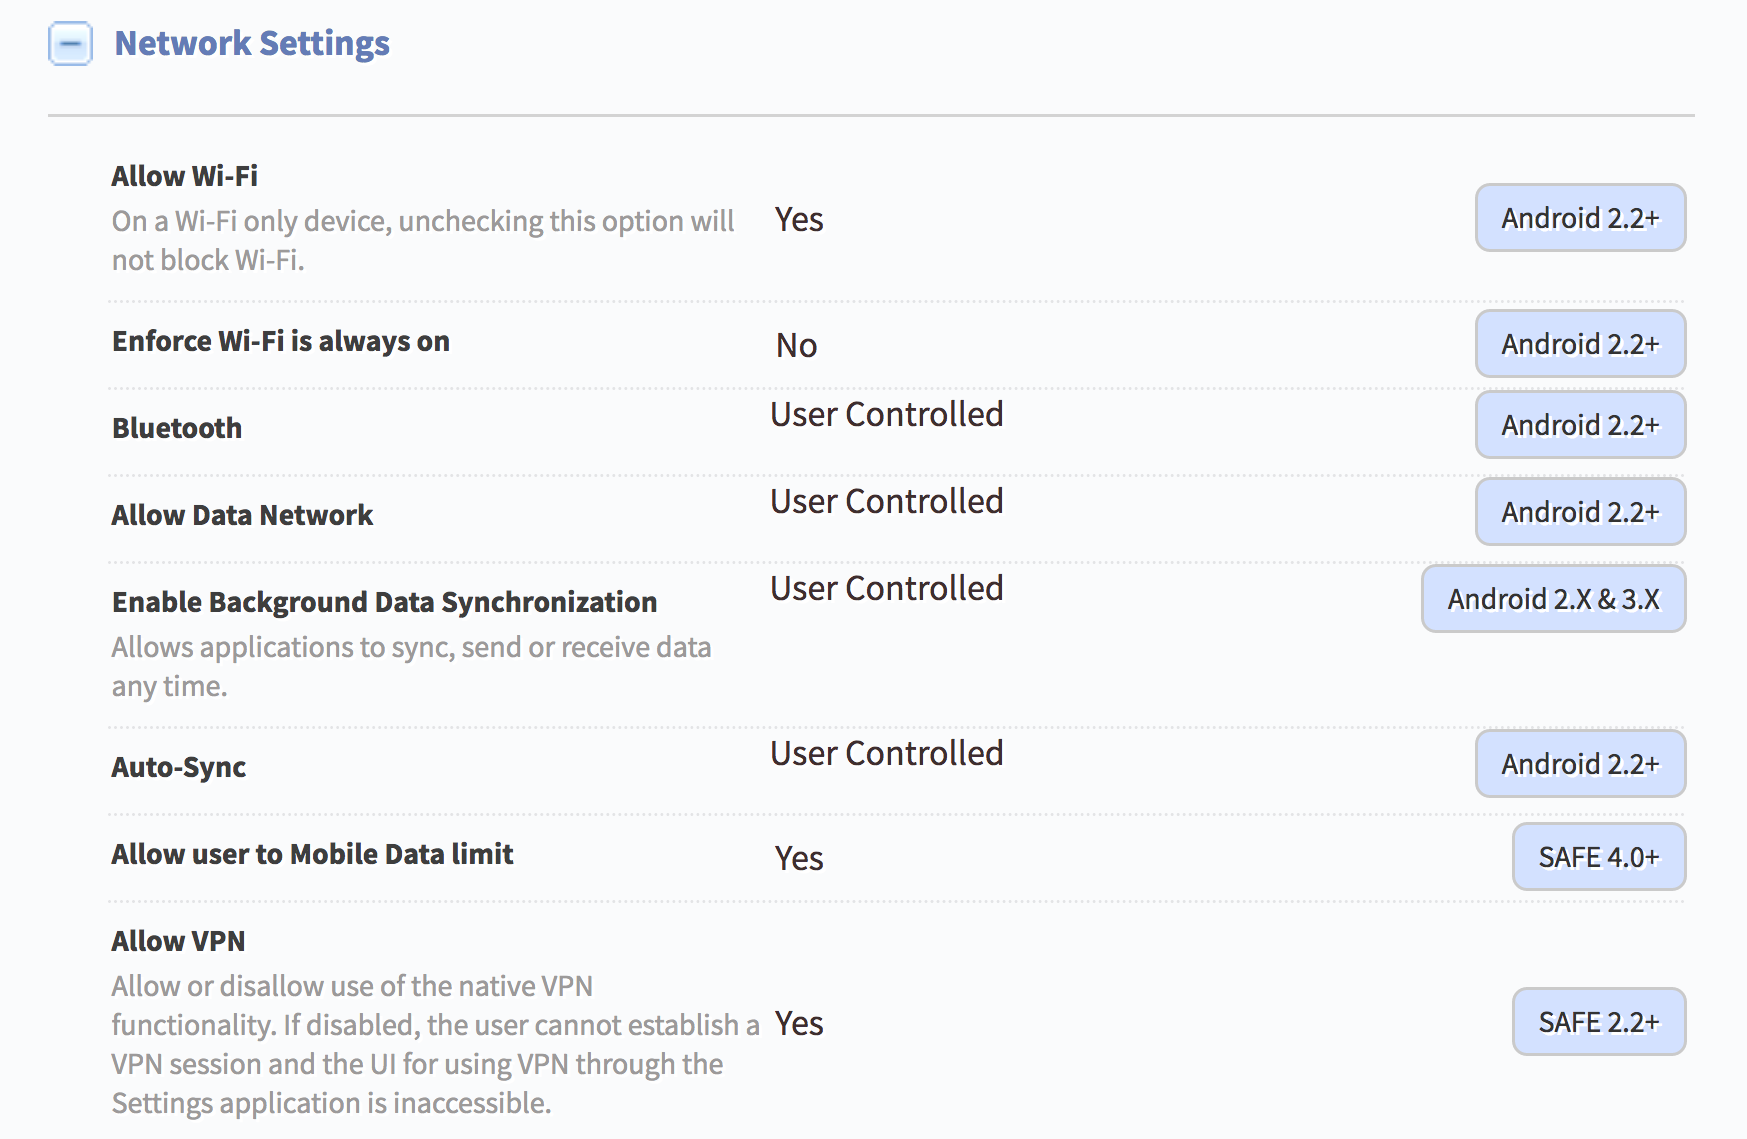
\includegraphics[width=\textwidth]{figures/maas360-policy.png}
  \caption{Policy settings in the MaaS360 MDM tool.}
  \label{fig:maas360-policy}
\end{figure}

As well as commercial \ac{MDM} tooling there are also research tools that look
at MDM software. Martinelli~\etal{}'s work looks at creating a dynamic
permissions manager, called UC-Droid. Their tool can alter what an app's Android
permissions are at run time based on policies~\cite{martinelli_enhancing_2016}.
The tool allows companies to reconfigure their apps depending on whether the
employee is at work, in a secret lab, or working out-of-hours. These kinds of
policies are more configurable than the geofenced based policies some \ac{MDM}
tools provide. Other work has looked at enforcing different policies based on
what roles an employee holds~\cite{costantino_towards_2013}. The work allowed a
company to verify the devices within their network and what servers and services
they could access. It also describes a mechanism for providing different users
with different policies.

Armando~\etal~developed BYODroid as a tool for enforcing BYOD policies through a
secure marketplace~\cite{armando_bring_2013}. Their tool allows companies to
distribute apps through a secure app~store~\cite{armando_enabling_2014}. The
store ensures apps meet policies through a combination of static analysis and
app rewriting with dynamic enforcement. Their policies are low level, based on
ConSpec~\cite{aktug_conspec_2008}, allowing checks based on Dalvik VM's state.
Using their tool, they implemented parts of a NATO Communications and
Information Agency policy relating to personal networks and data
management~\cite{armando_developing_2016}. Their work shows how the app-specific
sections of a BYOD policy can be check and enforced using tools. They did not
look at where the checks or policies come from, however.


\section{Modelling BYOD policies}

Each of the policies are split into a series of rules. A simple example is the
following example from the Sirens-company policy. The policy states that devices
may access various company resources. For each resource we create a SecPAL
assertion that states that a device can access it.

\begin{policyrule}{Sirens}
  Employees may use their mobile device to access the following company-owned resources:
  \newline $\bullet$ Email $\bullet$ Calendars $\bullet$ Contacts $\bullet$ Documents $\bullet$ Etc.
  \normalfont
  \begin{lstlisting}
'department' says Device:D canAccess('email').
'department' says Device:D canAccess('calendars').
'department' says Device:D canAccess('contacts').
'department' says Device:D canAccess('documents').
  \end{lstlisting}
\end{policyrule}

A more complex example can be taken from the NHS policy. Employees are not
allowed to call non-domestic, or premium rate numbers on company-owned
phones~\footnote{The NHS policy doesn't distinguish between company and
privately owned phones and applies to both.}, however an exception can be made
if approved by the appropriate manager. To implement this we have the default
rule that international calls are banned, a second rule stating that it is
allowed if an exemption is made, finally a third rule delegating the exemption
making process to the employee's manager.

\begin{policyrule}{NHS}
  All mobile devices will be configured for national access only. Premium/international calls will be barred.
  International call barring and roaming arrangements can be lifted for specific periods, to be stipulated on request, on approval of the relevant manager/budget holder.
  \normalfont
  \begin{lstlisting}
'nhs-trust' says Device canCall(TelephoneNumber:X)
  if Device isOwnedBy('nhs-trust'),
     X isNationalNumber, X isStandardRateNumber.

'nhs-trust' says Device canCall(TelephoneNumber:X)
  if Device isOwnedBy(Staff),
     Staff hasCallExemption.

'nhs-trust' says Manager can-say
  Staff hasCallExemption
  if Manager isManagerOf(Staff).
  \end{lstlisting}
\end{policyrule}

The occurrence of different types of predicate is shown in \autoref{tab:prefix}.
As before in \autoref{ssec:types} predicates The use of each is also split by
whether the predicate is a \emph{decision} made by the policy, or a
\emph{condition} for making that decision. \emph{Can} and \emph{must} decisions
feature in all policies excepting \emph{can} decisions in the Edinburgh policy,
in part due to the structure of the policy as discussed in
\autoref{sec:byod_policies}. This is expected, these are access control
decisions and reactions to events; both topics that existing MDM tools have
focused on implementing. \emph{Has} and \emph{is} predicates are the majority of
the conditions, but there are also decisions using them too.

\begin{table}\sffamily\small\centering
  \newcommand{\zilch}[0]{\small 0}
  \newcommand{\numpc}[2]{\small #2\% {\small(#2)}}
  \setlength{\tabcolsep}{1pt}
\begin{tabular}{ c  c c c c c c c c c }
\toprule
             & \multicolumn{4}{c}{Decision}                                                    && \multicolumn{4}{c}{Condition} \\
Policy       & \rb{Can}                     & \rb{Must}      & \rb{Has}       & \rb{Is}        && \rb{Can}      & \rb{Must}     & \rb{Has}        & \rb{Is}        \\
\midrule
SANS         & \numpc{26}{35}               & \numpc{22}{29} & \numpc{7 }{9 } & \numpc{20}{27} && \numpc{2 }{2} & \numpc{2 }{2} & \numpc{8 }{8}   & \numpc{81}{87} \\
HiMSS        & \numpc{6 }{21}               & \numpc{12}{41} & \numpc{9 }{31} & \numpc{2 }{7 } && \zilch        & \zilch        & \numpc{3 }{13}  & \numpc{20}{87} \\
NHS          & \numpc{13}{19}               & \numpc{18}{26} & \numpc{23}{33} & \numpc{16}{23} && \numpc{2 }{2} & \zilch        & \numpc{20}{19}  & \numpc{83}{83} \\
Sirens       & \numpc{12}{27}               & \numpc{20}{45} & \numpc{5 }{11} & \numpc{7 }{16} && \numpc{1 }{2} & \numpc{4 }{7} & \numpc{1 }{2}   & \numpc{50}{89} \\
Edinburgh    & \zilch                       & \numpc{2 }{18} & \numpc{9 }{82} & \zilch         && \numpc{2 }{7} & \numpc{2 }{7} & \numpc{15}{ 50} & \numpc{11}{37} \\
\bottomrule \\
\end{tabular}
\caption{Counts of predicate-types in each policy.}
\label{tab:prefix}
\end{table}

\section{Common Concerns and Checks}
\label{sec:common_concerns}

Analysing each of the policies common concerns become apparent.
A summary of predicates, with the same meaning, used in multiple policies by our translation is given in \autoref{tab:common}.

Acknowledgements, where individuals are asked to acknowledge other policies, and predicates linking devices to owners are used in all policies.
Most policies described rules for when device features should be enabled and disabled.
Configuring device features is a common feature to many MDM packages, but tracking what a user agrees to is not seen in leading MDM packages like MaaS360 or BES~\cite{rob_smith_magic_2016}.
Only 2 of the 5 policies had rules limiting what networks, servers, or access points a device could access;
  and only the two most complex policies had rules limiting what apps could be installed.
This is surprising as a common feature of MDM tools is controlling how devices and apps access networks.
Users have privacy preferences about apps~\cite{lin_modeling_2014}, but not all companies try to control what apps employees install.
Providing curated app stores and blacklisting apps is a feature common to many MDM programs.
Not all policies express rules about which apps to install, however.

\begin{table}\sffamily\footnotesize\centering
  \begin{tabular}{c c c c c c}
    \toprule                        \\
    Predicate                       & \rb{SANS} & \rb{HiMSS} & \rb{NHS} & \rb{Sirens} & \rb{Edinburgh} \\
    \midrule
    mustAcknowledged    &    \cmark & \cmark     &   \cmark & \cmark      &         \cmark \\
    hasAcknowledged     &    \cmark & \cmark     &   \cmark & \cmark      &         \cmark \\
    isOwnedBy           &    \cmark & \cmark     &   \cmark & \cmark      &         \cmark \\
    isDevice            &    \cmark & \cmark     &   \cmark & \cmark      &         \cmark \\
    mustDisable         &    \cmark &            &   \cmark & \cmark      &         \cmark \\
    isLost              &    \cmark & \cmark     &   \cmark & \cmark      &                \\
    isEmployee          &    \cmark &            &   \cmark & \cmark      &         \cmark \\
    isApp               &    \cmark & \cmark     &   \cmark & \cmark      &                \\
    isActivated         &    \cmark & \cmark     &   \cmark &             &         \cmark \\
    mustEnable          &    \cmark & \cmark     &          & \cmark      &                \\
    mustWipe            &           & \cmark     &   \cmark & \cmark      &                \\
    isEncrypted         &    \cmark &            &   \cmark &             &         \cmark \\
    hasMet              &    \cmark &            &   \cmark &             &         \cmark \\
    canMonitor          &    \cmark &            &   \cmark & \cmark      &                \\
    mustInform          &    \cmark &            &   \cmark &             &                \\
    isTelephoneNumber   &    \cmark &            &   \cmark &             &                \\
    isString            &           &            &   \cmark & \cmark      &                \\
    isSecurityLevel     &    \cmark & \cmark     &          &             &                \\
    isInstallable       &    \cmark &            &   \cmark &             &                \\
    isFeature           &    \cmark &            &          & \cmark      &                \\
    isData              &    \cmark &            &          & \cmark      &                \\
    isApprovedFor       &           & \cmark     &   \cmark &             &                \\
    isApproved          &    \cmark & \cmark     &          &             &                \\
    hasFeature          &           &            &   \cmark &             &         \cmark \\
    hasDevice           &           & \cmark     &   \cmark &             &                \\
    hasDepartment       &           & \cmark     &          &             &         \cmark \\
    canUse              &    \cmark &            &   \cmark &             &                \\
    canStore            &    \cmark & \cmark     &          &             &                \\
    canInstall          &    \cmark &            &   \cmark &             &                \\
    canConnectToServer  &    \cmark &            &   \cmark &             &                \\
    canConnectToNetwork &    \cmark &            &          & \cmark      &                \\
    canConnectToAP      &    \cmark & \cmark     &          &             &                \\
    canCall             &    \cmark &            &   \cmark &             &                \\
    canBackupTo         &           & \cmark     &          &             &         \cmark \\
    \bottomrule                     \\
  \end{tabular}
  \caption{Occurrences of predicates common to multiple policies.}
  \label{tab:common}
\end{table}


\section{BYOD idioms in AppPAL}

When examining the policies, two particular idioms occur in many policies: acknowledgements and delegation.
We describe both idioms in greater detail, and show how they can be implemented in AppPAL, below.
MDM tools and research have focussed so far on implementing restrictions on apps and devices~\cite{_ibm_????,armando_formal_2014,martinelli_enhancing_2016}.
Implementing these controls is a vital aspect of BYOD policies and all 5 of the policies we looked at had rules that described restrictions~(\autoref{tab:summary}).
Every policy also contained rules that required employees acknowledgements, however.
Only the SANS policy (which is configuration focussed) contained more rules that required restrictions than acknowledgements.
All the policies contained more rules featuring delegation relationships than functionality restrictions.
Restricting device functionality is tricky and important, but other aspects of BYOD policies are also worth attention.

\subsection{Delegation and Roles within Policies.}

Delegation is an important part of each of the policies.
Each of the policies describes through rules how separate entities may be responsible for making some decisions.
These rules can be a delegation to an employee's manager to authorize a decision (as in the NHS policy).
It could be to technical staff to decide what apps are part of a standard install (as in the sirens and SANS policies).

When translating the policies, the author of the policy is used as the primary speaker of the policy's rule (\autoref{tab:summary}).
For the \ac{HiMSS} policy, where the user states what they will do rather than the company stating what they must, the user is the primary speaker.
All the policies describe multiple entities that might make statements and delegate.

Some policies have more authorities, than others (\autoref{tab:principals}).
The NHS policy has various managers that approve decisions for their staff.
There are different groups that make decisions for the clinical and business halves of the business.
If a clinical user wishes to use an app with a patient they must seek approval from two policy groups, as well as their line manager.
Others make less use of different authorities.
In the Edinburgh policy, the records-management office states how a low or high risk must be configured.
There is no delegation to others to further specify aspects of the policy.
Delegation of responsibilities is an important part of BYOD policies.
MDM software seems largely to ignore it, however.
These tools instead allow IT staff to set fixed policies and push them to devices.
No further requesting of information is typically needed or required.

\begin{table}\centering\footnotesize\sffamily
  \begin{tabular}{c l l}
    \toprule
    \multirow{4}{*}{\rb{SANS}}       & Authorities         & 10                \\
                                     & Primary Authority   & company           \\
                                     & Technical Authority & it-department     \\
                                     & User Authority      & user              \\
    \midrule
    \multirow{4}{*}{\rb{HiMSS}}      & Authorities         & 3                 \\
                                     & Primary Authority   & user              \\
                                     & Technical Authority & xyz-health-system \\
                                     & User Authority      & department        \\
    \midrule
    \multirow{4}{*}{\rb{NHS}}        & Authorities         & 11                \\
                                     & Primary Authority   & nhs-trust         \\
                                     & Technical Authority & it-department     \\
                                     & User Authority      & staff             \\
    \midrule
    \multirow{4}{*}{\rb{Sirens}}     & Authorities         & 4                 \\
                                     & Primary Authority   & department        \\
                                     & Technical Authority & it-department     \\
                                     & User Authority      & employee          \\
    \midrule
    \multirow{4}{*}{\rb{Edinburgh}}  & Authorities         & 2                 \\
                                     & Primary Authority   & records-management\\
                                     & Technical Authority &                   \\
                                     & User Authority      & employee          \\
    \bottomrule                     \\
  \end{tabular}
  \caption{Summary of different authorities in BYOD policies.}
  \label{tab:principals}
\end{table}

When a policy decision requires input from a third-party delegation is used.
For example, an employee's manager has to authorise an app install.
The SecPAL \emph{can-say} statement is the basis for a delegation.
We can ask the HR department to state who is someone's manager.
\begin{lstlisting}
'company' says 'hr-department' can-say
  Employee:E hasManager(Employee:M).
\end{lstlisting}
If we wish to delegate to someone, we can add conditionals to the can-say statement that enforces any relationship between the delegating and delegated parties.
\begin{lstlisting}
'company' says Manager can-say
  Employee canInstall(App:A)
  if Employee hasManager(Manager).
\end{lstlisting}

\subsection{Acknowledgement.}

All the policies we looked at require their subjects to be aware and acknowledge certain rules or policies,
  and that the company may perform certain actions.
For example, the NHS and \ac{HiMSS} policies state that the organisation will wipe devices remotely to protect confidential information a user loses their device.
Both policies also say that employees would lose personal information if they had it on the device and the company needed to erase it.
The employee is required to be aware of this, and in the case of the \ac{HiMSS} policy, agree to hold the company harmless for the loss.

\begin{center}
  \noindent
  %\begin{minipage}{0.49\linewidth}
    \begin{policyrule}{HiMSS}
      I agree to hold XYZ Health System harmless for any loss relating to the
      administration of PDA/Smartphone connectivity to XYZ Health System systems
      including, but not limited to, loss of personal information stored on a
      PDA/Smartphone due to data deletion done to protect sensitive information
      related to XYZ Health System, its patients, members or partners.
      \normalfont
      \begin{lstlisting}
'xyz-health-system' says 'user' mustAcknowledged('data-loss-policy').
      \end{lstlisting}
    \end{policyrule}
  %\end{minipage}
  %\begin{minipage}{0.49\linewidth}
    \begin{policyrule}{NHS}
      Individuals who have personal data of any kind stored on a corporately
      issued mobile device must be aware that in the event of loss of the device
      the above data wipe will include removal of all personal data.
      \normalfont
      \begin{lstlisting}
'nhs-trust' says Staff:S can-say
  S hasAcknowledged('data-loss-policy').
'nhs-trust' says Staff:S mustAcknowledged('data-loss-policy').
      \end{lstlisting}
    \end{policyrule}
  %\end{minipage}
\end{center}

Both the SANS and the siren-company policies use acknowledgements to link to other sets of rules that employees should follow.
These policies are not further specified, and in the case of an acceptable use policy may be hard to enforce automatically.
The SANS policy requires that all employees follow an email security, acceptable use, and an eCommerce-security policy.
The Sirens policy expects an employee to use their devices ethically and abide by an acceptable use policy.

\begin{policyrule}{SANS}
  Users MUST agree to the email security/acceptable use policy and eventually to the eCommerce security policy.
  \begin{lstlisting}
'company' says Employee:U mustAcknowledged('email-security').
'company' says Employee:U mustAcknowledged('acceptable-use').
'company' says Employee:U mustAcknowledged('ecommerce-security').
  \end{lstlisting}
\end{policyrule}
\begin{policyrule}{Sirens}
  The employee is expected to use his or her devices in an ethical manner at all times and adhere to the company's acceptable use policy.
  \begin{lstlisting}
'department' says Employee:E mustAcknowledged('acceptable-use').
  \end{lstlisting}
\end{policyrule}

When there is a (usually separate) set of rules and concerns employees should be aware of acknowledgements are used.
The company may not have wish to enforce these separate rules automatically, however.
For instance, a company may have an ethical policy that says employees should not use devices for criminal purposes.
The company is not interested in, or capable of, defining what is criminal.
They trust their employees to make the right decision and to be aware of the rules.

To implement these in AppPAL, a policy author creates two rules:
  the first stating their employees must have acknowledged the policy,
  the second delegating the acceptance of the policy to the employee themselves.
\begin{lstlisting}
'company' says Employee:E mustAcknowledged('policy').
'company' says Employee:E can-say
  E hasAcknowledged('policy').
\end{lstlisting}

%\comment{
%  \bibliography{thesis}
%}
\end{document}


%%% Local Variables:
%%% mode: latex
%%% TeX-master: "../ch5"
%%% End:
